% !TEX options=--shell-escape
\documentclass[usenames,dvipsnames,9pt]{beamer}

\makeatletter
\def\input@path{{../support/beamer-template/}}
\makeatother

\usepackage{../support/beamer-template/beamerthememetropolis}

\usepackage[utf8]{inputenc}
\usepackage[czech]{babel}
\selectlanguage{czech}

\usepackage{hyperref}
\usepackage{fontawesome}
\usepackage{minted}
\usepackage{mathtools}
\usepackage{tabularx}
\usepackage{smartdiagram}
\usepackage{amssymb}
\usepackage{qrcode}

% Commands shared between most of the tutorial slides

% Homework deadlines
\newcommand{\hwVIIdeadline}{10. 5. 2020}



% Download icon and text with link relative to the root of the courseware site
\newcommand{\download}[1]{\hfill\faDownload\hspace{5pt}\href{https://cw.fel.cvut.cz/wiki/_media/courses/be4m36mas/#1}{\tt #1}\\[1.3em]}

% Draw eye icon
\newcommand{\see}[1]{\faEye\hspace{5pt}#1}

\newcommand{\sep}{\hspace{10pt}/\hspace{10pt}}

\def\Ipe#1{\def\IPEfile{#1}\input{#1}}

% Draw pacman icon
\newcommand{\pacman}[1]{\tikz[baseline=.1em,scale=.6]{
    \useasboundingbox (.02,0) rectangle (.6,.6);
  \draw [fill=#1] (.3,.3) -- ++(25:.3) arc (+25:+335:.3) -- cycle;

}}

% Draw ghost icon
\newcommand{\ghost}[1]{\tikz[baseline=.1em,scale=.5]{
  \draw [fill=#1] (0,0) -- (0,.5) arc (+180:0:.3) -- (.6,0) --
  (.5,.15) -- (.4,0) -- (.3,.15) -- (.2,0) -- (.1,.15) -- cycle;
    \coordinate (eye) at (360*rand:.03);
    \foreach \x in {.17,.43}{
      \fill[white] (\x,.5) circle[radius=.1];
      \fill[black] (\x,.5) ++(eye) circle[radius=.05];
    }
}}

\newcommand{\desc}[2]{
  #1

  \vspace{-0.6em}
  \hfill\begin{minipage}{0.9\linewidth}
    #2
  \end{minipage}

  \vspace{0.2em}
}

\newcommand{\redc}{\tikz\draw[red,fill=red] (0,0) circle (.5ex);}

\newcommand{\greenc}{\tikz\draw[green,fill=green] (0,0) circle (.5ex);}


% Default url for generating QR code with feedback form.
\newcommand{\defaultfeedbackurl}{https://forms.gle/vwbWazEu14w1Kf487}

% Generate frame with QR code to a feedback form.
\newcommand{\framefeedback}[1][\defaultfeedbackurl]{
  \begin{frame}[standout]
    \begin{minipage}{0.4\linewidth}
      \begin{center}
        \textbf{\LARGE Díky za pozornost!}
      \end{center}

      \vspace{3em}

      \raggedleft\small Budeme rádi za Vaši\\zpětnou vazbu! $\rightarrow$
    \end{minipage}
    \hfill
    \begin{minipage}{0.5\linewidth}
      \vspace{4em}
      \centering\qrcode[height=\linewidth]{#1}\\
      \vspace{0.8em}
      \url{#1}
    \end{minipage}
  \end{frame}
}

\title{Paralení programování pro vícejádrové stroje s použitím OpenMP}
%\subtitle{Organizace předmětu a seznámení se s paralelizací}
\date{}
\institute{B4B36PDV -- Paralelní a distribuované výpočty}

\metroset{block=fill}

\begin{document}
\maketitle

\begin{frame}
  Minulé cvičení:
  \begin{center}
    \Large\emph{``Vlákna a jejich synchronizace v C++ 11...''}
  \end{center}
  \pause
  \vspace{1.5em}
  
  Programování vícevláknových aplikací ručně může být dřina. Proč znovu objevovat kolo, když mužeme použít hotové řešení?

  \pause
  \vspace{2.5em}
  Dnešní menu: \hspace{10pt} \huge OpenMP
\end{frame}

\begin{frame}
  \frametitle{Osnova}
  \begin{itemize}
    \item Opakování z minulého cvičení
    \item Úvod do OpenMP
    \item Paralelní bloky se sdílenou pamětí a synchronizace
    \item Redukce s OpenMP
    \item Rozvrhování výpočtu v OpenMP\\[1.5em]
    \item Zadání druhé domácí úlohy
  \end{itemize}
\end{frame}

\section{Opakování z minulého cvičení}
\begin{frame}[standout]
  \Huge
  \url{http://goo.gl/a6BEMb}
\end{frame}

% pripomenuti - prehled, co je openmp
\section{Co je OpenMP?}
\begin{frame}
  \frametitle{OpenMP: Přehled}
  \begin{itemize}
    \item API pro psání vícevláknových aplikací se sdílenou pamětí
    \item Sada directiv, proměnných prostředí a rutin pro kompilátor a programátory
    \item Ulehčuje psaní vícevláknových aplikací v C/C++ a Fortran na většině platform s podporou většiny instrukčních sad a operačních systémů
  \end{itemize}
  \pause
  {\small
  Jako základní referenční příručku můžete použít \url{https://msdn.microsoft.com/en-us/library/tt15eb9t.aspx}}
\end{frame}

% test prostredi + komentare, co veci znamenaji - postupny vypis
{\setbeamertemplate{frame footer}{\see{{\tt test.cpp} \sep {\tt make test\_openmp}}}
\begin{frame}[fragile]
  \frametitle{Otestujte si své prostředí}

  \desc{\mintinline{c}{omp_get_num_procs()}}{Počet procesorů, které OpenMP využívá v době volání funkce}

  \desc{\mintinline{c}{omp_get_num_threads()}}{Počet vláken, které OpenMP využívá v době volání funkce}

  \desc{\mintinline{c}{omp_get_max_threads()}}{Maximální počet vláken, které OpenMP může využít}

  \desc{\mintinline{c}{omp_in_parallel()}}{Vrací nenulovou hodnotu, pokud jsme uvnitř paralelního bloku}

  \desc{\mintinline{c}{omp_get_nested()}}{Vrací nenulu, pokud je povoleno vnořování paralelních bloků}

  \pause

  \vspace{1em}

  {\small
  Detailní přehled metod s ukázkami na \url{https://msdn.microsoft.com/en-us/library/k1h4zbed.aspx}.}
\end{frame}
}

% vypocet integralu - jak muzeme vypocitat
\section{Cvičení: Numerická integrace}

{\setbeamertemplate{frame footer}{\see{{\tt integrate.cpp},\ \ \ {\tt main.cpp} \sep {\tt make main}}}
\begin{frame}[fragile]
  \frametitle{Numerická integrace}
  
  \begin{figure}
    \centering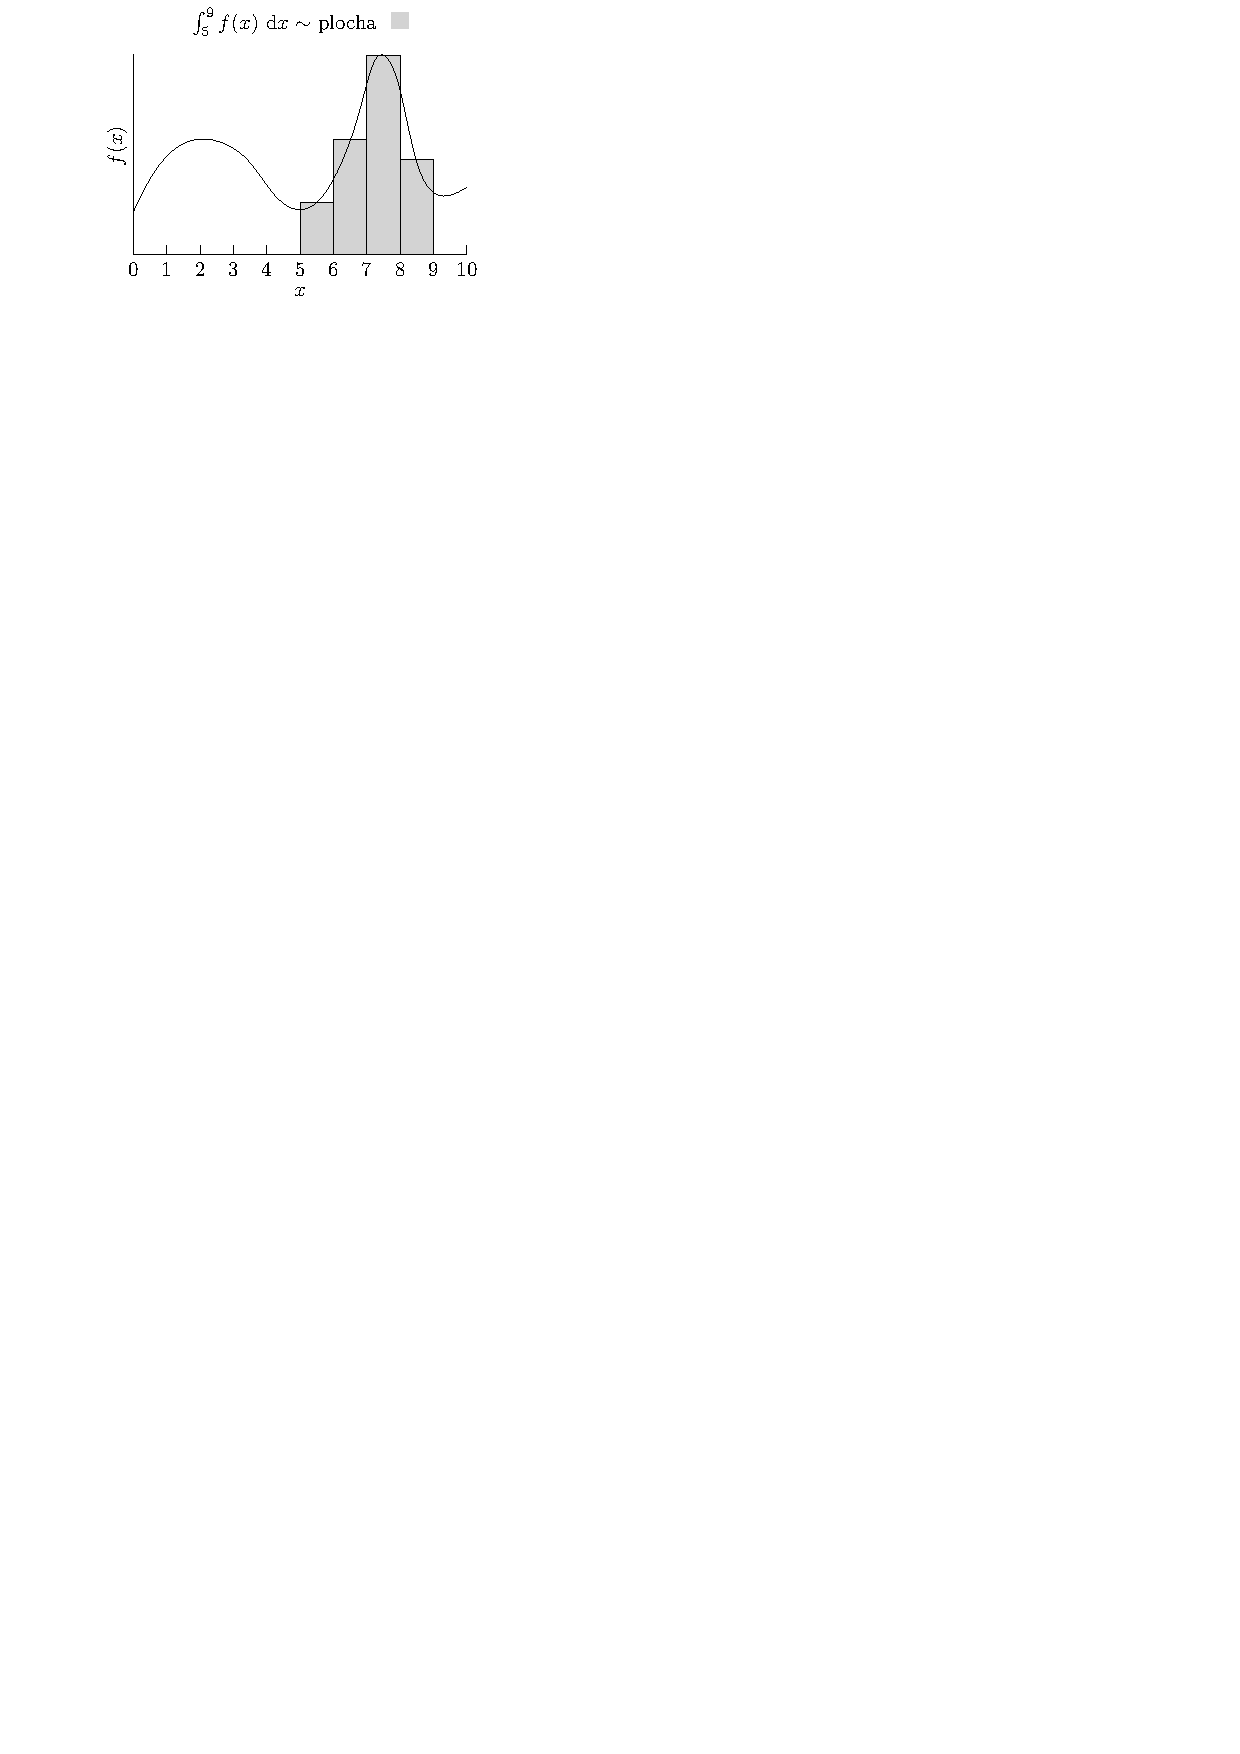
\includegraphics{figs/integral.pdf}
  \end{figure}

  \begin{minted}{c}
    double integrate(
      std::function<double(double)> integrand,
      double a, double step_size, int step_count);
  \end{minted}
\end{frame}

% dve funkce - prehled, vytvorte sekvencni verzi, zadani - sekvencni implementace.
\begin{frame}[fragile]
  \begin{block}{Doimplementujte sekvenční verzi numerické integrace}
    Doimplementujte tělo metody \texttt{integrate\_sequential} v souboru \texttt{integrate.cpp}.
    Použijte obdélníkovou metodu, kdy jako ``výšku'' obdélníku použijete hodnotu funkce uprostřed intervalu.

    \desc{\texttt{integrand}}{Funkce, kterou máte za úkol numericky zintegrovat}
    \desc{\texttt{a}}{Dolní mez integrálu}
    \desc{\texttt{step\_size}}{Velikost kroku (šířka obdélníku)}
    \desc{\texttt{num\_steps}}{Počet kroků (horní mez je \texttt{a + step\_size * step\_count})}
  \end{block}

  % jake jsou problemy, pokud budeme chtit paralelizovat? jak byste to resili na zaklade toho, co znate z minula?
  \pause
  \vspace{0.2em}
  \begin{center}
    \Large
    Jaké problémy budeme mít, pokud budeme chtít tento sekvenční kód paralelizovat?
  \end{center}
\end{frame}
}

\section{Alternativy k mutexům a atomickým proměným v OpenMP}

\begin{frame}[fragile]
  \frametitle{\texttt{\#pragma omp parallel}}
  \begin{minted}{c}
int num_threads = 0;
#pragma omp parallel
{
  // Zde jsme vytvorili tym vlaken, ktera vykonavaji
  // nasledujici kod
  num_threads += 1; 
}
  \end{minted}

  \pause

  \begin{center}
    \Large Jaký bude výsledek?
  \end{center}
\end{frame}

% ukazka na critical
\begin{frame}[fragile]
  \frametitle{\texttt{\#pragma omp critical} \hspace{10pt} (``mutex'')}
  \begin{minted}{c}
int num_threads = 0;
#pragma omp parallel
{
  // Zde muze byt vice vlaken soucasne...

  #pragma omp critical
  {
    // ..,ale inkrementaci provadi vzdy maximalne
    // jedno vlakno
    num_threads += 1; 
  }

  // Zde opet muze byt vice vlaken soucasne
}
  \end{minted}
\end{frame}

{\setbeamertemplate{frame footer}{\see{{\tt integrate.cpp},\ \ \ {\tt main.cpp} \sep {\tt make main}}}
\begin{frame}
  \begin{block}{Doimplementujte metodu \texttt{integrate\_omp\_critical}}
    Doimplementujte metodu \texttt{integrate\_omp\_critical} v \texttt{integrate.cpp}.
    Využijte k tomu \texttt{\#pragma omp parallel} a \texttt{\#pragma omp critical}.

    \emph{Tip:}
    Po spuštění vláken v bloku \texttt{\#pragma omp parallel} si můžete napočítat rozsahy indexů, které jednotlivá vlákna budou zpracovávat (viz \texttt{decrypt\_threads\_4} z minulého cvičení).
    Pro zjištění indexu aktuálního vlákna použijte metodu \texttt{omp\_get\_thread\_num()}.
    Zjistit celkový počet vláken lze pomocí \texttt{omp\_get\_num\_threads()}.
  \end{block}
\end{frame}
}

% ukazka na atomic
\begin{frame}[fragile]
  \frametitle{\texttt{\#pragma omp atomic}}
  Na minulém cvičení jsme si ukázali, že mutexy mohou být pomalé.\\
  \textbf{Opravdu pomalé.}
  \begin{itemize}
    \item[\ \ \ \ \ $\rightarrow$] Jednoduché operace nad jednou proměnnou lze řešit \emph{hardwarovým} zámkem -- provedením atomické operace
  \end{itemize}

  \vspace{1.5em}

  \begin{minipage}{0.4\linewidth}
    \begin{minted}{c}
int num_threads = 0;
#pragma omp parallel
{
  #pragma omp atomic
  num_threads += 1;
}
    \end{minted}
  \end{minipage}
  \begin{minipage}{0.59\linewidth}
    Ne všechny operace lze provést atomicky!

    \vspace{0.5em}

    Typicky pouze: \texttt{x++}, \texttt{x--}, \texttt{++x}, \texttt{--x} \\
    a \texttt{x} \emph{OP}\texttt{= expr}, kde
    \vspace{-0.4em}
    \begin{center}
      \emph{OP} $\in \lbrace$
      \mintinline{c}{+}, 
      \mintinline{c}{-}, 
      \mintinline{c}{*}, 
      \mintinline{c}{/}, 
      \mintinline{c}{&}, 
      \mintinline{c}{^}, 
      \mintinline{c}{|}, 
      \mintinline{c}{<<}, 
      \mintinline{c}{>>}
      $\rbrace$
    \end{center}

    \begin{itemize}
      \item[\faThumbsOUp] Pokud kompilátor nemá k dispozici danou atomickou operaci, použije záložní plán: mutex.
    \end{itemize}
  \end{minipage}
\end{frame}

{\setbeamertemplate{frame footer}{\see{{\tt integrate.cpp},\ \ \ {\tt main.cpp} \sep {\tt make main}}}
\begin{frame}
  \begin{block}{Doimplementujte metodu \texttt{integrate\_omp\_atomic}}
    Doimplementujte metodu \texttt{integrate\_omp\_atomic} v \texttt{integrate.cpp}.
    Místo kritické sekce využijte \texttt{\#pragma omp atomic}.
    Jakého zrychlení touto úpravou dosáhneme?
  \end{block}
\end{frame}
}

\section{Redukce v OpenMP}

% ukazka na redukce
\begin{frame}[fragile]
  \frametitle{Redukce v OpenMP}

  To samé lze ale udělat elegantněji a efektivněji:
  \begin{minted}{c}
int num_threads = 0;
#pragma omp parallel reduction(+:num_threads)
{
  num_threads += 1; 
}
  \end{minted}

  OpenMP pak zajistí, že se částečné výsledky \emph{lokálních} proměnných \texttt{num\_threads} po konci bloku posčítají

  \vspace{1em}\hrule\vspace{1em}

  Následující ``operátory'' jsou podporované (OpenMP verze 3+):
  \begin{itemize}
    \item Aritmetické: \mintinline{c}{+}, \mintinline{c}{*}, \mintinline{c}{-}, \mintinline{c}{max}, \mintinline{c}{min}
    \item Logické: \mintinline{c}{&}, \mintinline{c}{&&}, \mintinline{c}{|}, \mintinline{c}{||}, \mintinline{c}{^}
  \end{itemize}
\end{frame}

% uloha, proc nam uloha neskaluje tak dobre v druhem pripade? co udelat, aby se zlepsil vykon?
{\setbeamertemplate{frame footer}{\see{{\tt integrate.cpp},\ \ \ {\tt main.cpp} \sep {\tt make main}}}
\begin{frame}[fragile]
  \begin{block}{Doimplementujte metodu \texttt{integrate\_omp\_reduction}}
    Doimplementujte tělo metody \texttt{integrate\_omp\_reduction} v souboru \texttt{integrate.cpp}.
    Nahraďte \texttt{\#pragma omp atomic} redukcí.
  \end{block}
\end{frame}
}

\begin{frame}[fragile]
  \frametitle{\texttt{\#pragma omp parallel for}}

  Kód s redukcí lze napsat ještě jednodušeji.

  Rozsahy pro vlákna si nemusíme počítat ručně a můžeme práci nechat na OpenMP:

  \begin{minted}{c}
double acc = 0.0;

#pragma omp parallel for reduction(+:acc) //schedule(static)
for(int i = 0 ; i < step_count ; i++) {
  const double cx = a + (2*i + 1.0)*step_size/2;
  acc += integrand(cx)*step_size;
}
return acc;
  \end{minted}
\end{frame}

\begin{frame}
  \begin{center}
    \Large
    Proč při integraci funkce $f(x)=x$ \\ dosahujeme většího zrychlení?
  \end{center}

  \pause\vspace{1.5em}

  Výpočet $f(x)=x$ trvá konstantní dobu a práce je tak mezi vlákna rozdělena rovnoměrně.

  To neplatí o funkci $f(x)=\int_0^{0.001x^2} \sin(p) \ \mathrm{d}p$, kterou aproximujeme numerickou integrací s proměnlivým počtem kroků.
\end{frame}

{\setbeamertemplate{frame footer}{\see{{\tt integrate.cpp},\ \ \ {\tt main.cpp} \sep {\tt make main}}}
\begin{frame}[fragile]
  \begin{block}{Doimplementujte metodu \texttt{integrate\_omp\_for\_dynamic}}
    Doimplementujte tělo metody \texttt{integrate\_omp\_for\_dynamic}.
    Statické rozvrhování \texttt{schedule(static)} nahraďte dynamickým \texttt{schedule(dynamic)}.
    Jaký má tato volba dopad na rychlost numerické integrace $f(x)=x$ a $f(x)=\int_0^{0.001x^2} \sin(p) \ \mathrm{d}p$?
  \end{block}
\end{frame}
}

% ukazka schedulingu, typy s vysvetlenim 
\begin{frame}[fragile]
  \frametitle{\texttt{\#pragma omp parallel for \underline{schedule}}}
  Obecná syntaxe (možno použít i další parametry jako např. \texttt{reduction}):
  \begin{minted}{c}
  #pragma omp parallel for schedule(type[,chunk_size])
  \end{minted}

  \pause

  \texttt{chunk\_size} udává minimální velikost bloku, se kterým se plánuje, např:
  \begin{minted}{c}
  #pragma omp parallel for schedule(dynamic,16)
  \end{minted}
  zajistí, že si vlákno po dokončení práce na aktuálním bloku dat řekne o další blok o 16 prvcích.

  \pause

  \begin{itemize}
    \item dynamic - vlákna si \emph{dynamicky} alokují bloky, které mají počítat
    \item guided - \emph{dynamické} plánování, kde se velikost bloků v průběhu výpočtu zmenšuje
    \item static - každé vlákno má svůj blok přiřazený napevno (když skončí dříve, musí čekat)
    \item runtime - rozhodnuto za běhu na základě nastavení prostředí \\ {\tt (export OMP\_SCHEDULE="dynamic, 100")}
  \end{itemize}
\end{frame}

\section{Zadání druhé domácí úlohy}


% TODO - domaci uloha
\begin{frame}
  \frametitle{Paralelní suma vektoru}
  
V 2. domácí úloze si budete moct vyzkoušet, že úspěšnost různých způsobů paralelizace {\bf závisí} do značné míry na {\bf vstupních datech}.

\vspace{1.5em}

Na vstupu dostanete vektor složený z vektorů náhodně generovaných čísel. 

\vspace{1.5em}

Vaším úkolem je čísla v každém vektoru {\bf sečíst} a tento součet vložit do vektoru s řešením na index odpovídající pořadí vektoru, který jste sčítali.
   
  
  

\end{frame}

% TODO - domaci uloha
\begin{frame}
  \frametitle{Paralelní suma vektoru}
  Doimplementujte metody v \texttt{SumsOfVectors.cpp} a zajistěte, že
  \begin{enumerate}
    \item Výpočet sum je paralelní a každá metoda vrací korektní výsledky
    \item Metody využívají požadované způsoby paralelizace
  \end{enumerate}
  
  \pause\vspace{1.5em}
  
  Za spravné výsledky na každé ze {\bf čtyř} datových sad dostanete 2b.

\end{frame}

% Frame with the feedback QR code 
\framefeedback{}

\end{document}
